%\documentclass[11pt,table]{beamer}
\documentclass[11pt,handout]{beamer}
\mode<presentation>
\usepackage{etex}
\usepackage{graphicx}
\usepackage{epstopdf}
\usepackage[english]{babel}
\usepackage{tabularx}
\usepackage{booktabs}
\usepackage{mathrsfs}
\usepackage{multicol}
\usepackage{bm}
\usepackage{subcaption}
\usepackage{wrapfig}
\usepackage{dcolumn}
\usepackage{threeparttable}
\usepackage{booktabs}
\usepackage{bbm}
\usepackage{amsmath,dsfont,listings}
\usepackage{amssymb}
\usepackage{rotating}
\usepackage{multirow}
\usepackage[authoryear]{natbib}
\usepackage{circledsteps}
\usepackage{tikz}
\usetikzlibrary{arrows,decorations.pathmorphing,backgrounds,fit,positioning,shapes.symbols,chains}
\setbeamertemplate{section in toc}[sections numbered]
\setbeamertemplate{caption}[numbered]

\bibliographystyle{Econometrica}

\setbeamersize{text margin right=3.5mm, text margin left=7.5mm}  % text margin
\setbeamersize{sidebar width left=0cm, sidebar width right=0mm}
\setbeamertemplate{sidebar right}{}
\setbeamertemplate{sidebar left}{}

\definecolor{text-grey}{rgb}{0.45, 0.45, 0.45} % grey text on white background
\definecolor{bg-grey}{rgb}{0.66, 0.65, 0.60} % grey background (for white text)
\definecolor{fu-blue}{RGB}{0, 51, 102} % blue text
\definecolor{fu-green}{RGB}{153, 204, 0} % green text
\definecolor{fu-red}{RGB}{204, 0, 0} % red text (used by \alert)

\setbeamertemplate{frametitle}{%
    \vskip-30pt \color{text-grey}\large%
    \begin{minipage}[b][23pt]{80.5mm}%
    \flushleft\insertframetitle%
    \end{minipage}%
}

\setbeamertemplate{navigation symbols}{} 

%%% begin title page
\setbeamertemplate{title page}{
\vskip2pt\hfill
\vskip6pt\hskip3pt

% set the title and the author
\vskip14pt
\parbox[top][1.35cm][c]{11cm}{\LARGE\color{text-grey} Econome\textcolor{red1}{tricks}: \inserttitle \\[1ex] \small \quad \\[3ex]}
\vskip11pt
\parbox[top][1.35cm][c]{11cm}{\small Trick 06: \insertsubtitle \\[2ex] \insertauthor \\[1ex]}
}
%%% end title page

%%% colors
\usecolortheme{lily}
\setbeamercolor*{normal text}{fg=black,bg=white}
\setbeamercolor*{alerted text}{fg=fu-red}
\setbeamercolor*{example text}{fg=fu-green}
\setbeamercolor*{structure}{fg=fu-blue}

\setbeamercolor*{block title}{fg=white,bg=black!50}
\setbeamercolor*{block title alerted}{fg=white,bg=black!50}
\setbeamercolor*{block title example}{fg=white,bg=black!50}

\setbeamercolor*{block body}{bg=black!10}
\setbeamercolor*{block body alerted}{bg=black!10}
\setbeamercolor*{block body example}{bg=black!10}

\setbeamercolor{bibliography entry author}{fg=fu-blue}
\setbeamercolor{bibliography entry journal}{fg=text-grey}
\setbeamercolor{item}{fg=fu-blue}
\setbeamercolor{navigation symbols}{fg=text-grey,bg=bg-grey}
%%% end colors

%%% headline
\setbeamertemplate{headline}{
\vskip30pt
}
%%% end headline

%%% footline
\newcommand{\footlinetext}{
%\insertshortinstitute, \insertshorttitle, \insertshortdate
}
\setbeamertemplate{footline}{
\vskip2pt
\hfill \raisebox{-1pt}{\usebeamertemplate***{navigation symbols}}
\hfill \insertframenumber\hspace{10pt}
\vskip4pt
}
%%% end footline

%%% settings for listings package
\lstset{extendedchars=true, showstringspaces=false, basicstyle=\footnotesize\sffamily, tabsize=2, breaklines=true, breakindent=10pt, frame=l, columns=fullflexible}
\lstset{language=Java} % this sets the syntax highlighting
\lstset{mathescape=true} % this switches on $...$ substitution in code
% enables UTF-8 in source code:
\lstset{literate={�}{{\"a}}1 {�}{{\"o}}1 {�}{{\"u}}1 {�}{{\"A}}1 {�}{{\"O}}1 {�}{{\"U}}1 {�}{\ss}1}
%%% end listings

\usepackage{concmath}
\usepackage{xcolor}
\definecolor{red1}{RGB}{206, 17, 38}
\definecolor{blue1}{RGB}{16, 118, 208}
\definecolor{gray1}{RGB}{117, 115, 115}
\usepackage{hyperref}

\def\beX{\begin{itemize}}
\def\beXX{\begin{itemize}}
\def\beXXX{\begin{itemize}}
\def\beXXXX{\begin{itemize}}
\def\eeX{\end{itemize}}
\def\eeXX{\end{itemize}}
\def\eeXXX{\end{itemize}}
\def\eeXXXX{\end{itemize}}
\newtheorem{proposition}{Proposition}
\newtheorem{assumption}{Definition}


\title[]{Short guides to econometrics}
\subtitle[]{The Maximum Likelihood Estimator}
\author[D. Rostam-Afschar]{\textcolor{gray1}{Davud Rostam-Afschar (Uni Mannheim)}}
\date[]{\today}
\subject{Econometrics}
\renewcommand{\footlinetext}{\insertshortinstitute, \insertshorttitle, \insertshortdate}
\hypersetup{
    bookmarks=false,
    unicode=false,
    pdftoolbar=false,
    pdffitwindow=true,
    pdftitle={Short Guides to Econometrics: The Maximum Likelihood Estimator},
    pdfauthor={Davud Rostam-Afschar},
    pdfsubject={Maximum Likelihood Estimator},
    pdfkeywords={ML, sampling error, consistency, asymptotic normality, asymptotic efficiency},
    pdfnewwindow=true,
}
\def\sym#1{\ifmmode^{#1}\else\(^{#1}\)\fi}

\begin{document}

\begin{frame}[plain]
  \titlepage
\end{frame}

% --------------------------------------------------- Slide --
\begin{frame}
	\frametitle{Content}
	\tableofcontents[]
\end{frame}


\section{From Probability to Likelihood}

\begin{frame}{The Likelihood Principle}
Suppose you have three credit cards. You forgot, which has money on it or not. Thus, the number credit cards with money, call it $\theta$, might be 0, 1, 2, or 3. You can try your cards 4 times at random to check if you can make a payment.\\[2ex]
The checks are random variables $y_1, y_2, y_3,$ and $y_4$. They are
$$y_i= \begin{cases}
			      1, & \text{if the $i$th card has money on it,}\\
            0, & \text{otherwise}.
		 \end{cases}$$

Since you chose $y_i$'s uniformly, they are i.i.d. and $y_i\sim Bernoulli(\theta/3)$. After checking, we find $y_1=1,y_2=0,y_3=1,y_4=1$. We observe 3 cards with money and 1 without.\\[2ex]

The number credit cards with money could still be 0, 1, 2, or 3.\\ \textbf{Which is most likely?}
\end{frame}

\begin{frame}{From Probability to Likelihood}
You could test for the true $\theta_0$ in many samples. Conversely, you can check each possible value of $\theta$ to find the probability of observing the sample $(y_1=1,y_2=0,y_3=1,y_4=1)$.\\[2ex]

Since $y_i\sim Bernoulli(\theta /3)$, we have $$Prob(y_i=y)=\begin{cases}
			      \theta/3, & \text{for } y=1,\\
            1-\theta/3, & \text{for } y=0.
		 \end{cases}$$

Since $y_i$'s are independent, the joint PMF of $y_1, y_2, y_3,$ and $y_4$ can be written as
\begin{align}
&Prob(y_1=y,y_2=y,y_3=y,y_4=y|\theta)=\nonumber\\
&Prob(y_1)Prob(y_2)Prob(y_3)Prob(y_4).\nonumber
\end{align}
This depends on $\theta$, and is called \textbf{likelihood function}:
\begin{align}
&L(\theta|y_i)=Prob(y_1=1,y_2=0,y_3=1,y_4=1,\theta)=\nonumber\\
&\theta/3(1-\theta/3)\theta/3\theta/3=(\theta/3)^3(1-\theta/3).\nonumber
\end{align}
\end{frame}

\begin{frame}{The Likelihood Principle}

Values of the Likelihood $L(\theta|y_i)$ for different $\theta$
\begin{table}
\centering
{
\begin{footnotesize}
\begin{tabular}{@{\extracolsep{4pt}}l*{5}{c}}
\toprule
Trial & 1 & 2 & 3 & 4 \\
\midrule
$\theta$ & 0 & 1 & 2 & 3\\
$Prob(\cdot)$ & 0.0000 & 0.0247 & 0.0988 & 0.0000\\
\bottomrule
\end{tabular}
\end{footnotesize}
}
\end{table}

The probability of the observed sample for $\theta=0$ and $\theta=3$ is zero. This makes sense because our sample included both cards with and without money. The observed data is most likely to occur for $\theta=2$.\\[2ex]

\textbf{Likelihood principle}: choose $\theta$ that maximizes the likelihood of observing the actual sample to get an estimator for $\theta_0$.

The likelihood is the probability from 
\begin{itemize}
	\item probability mass function if discrete
	\item probability distribution function if continuous
\end{itemize}



\end{frame}

\begin{frame}{From Likelihood to Log-Likelihood}

\begin{figure}[H]
\begin{center}
{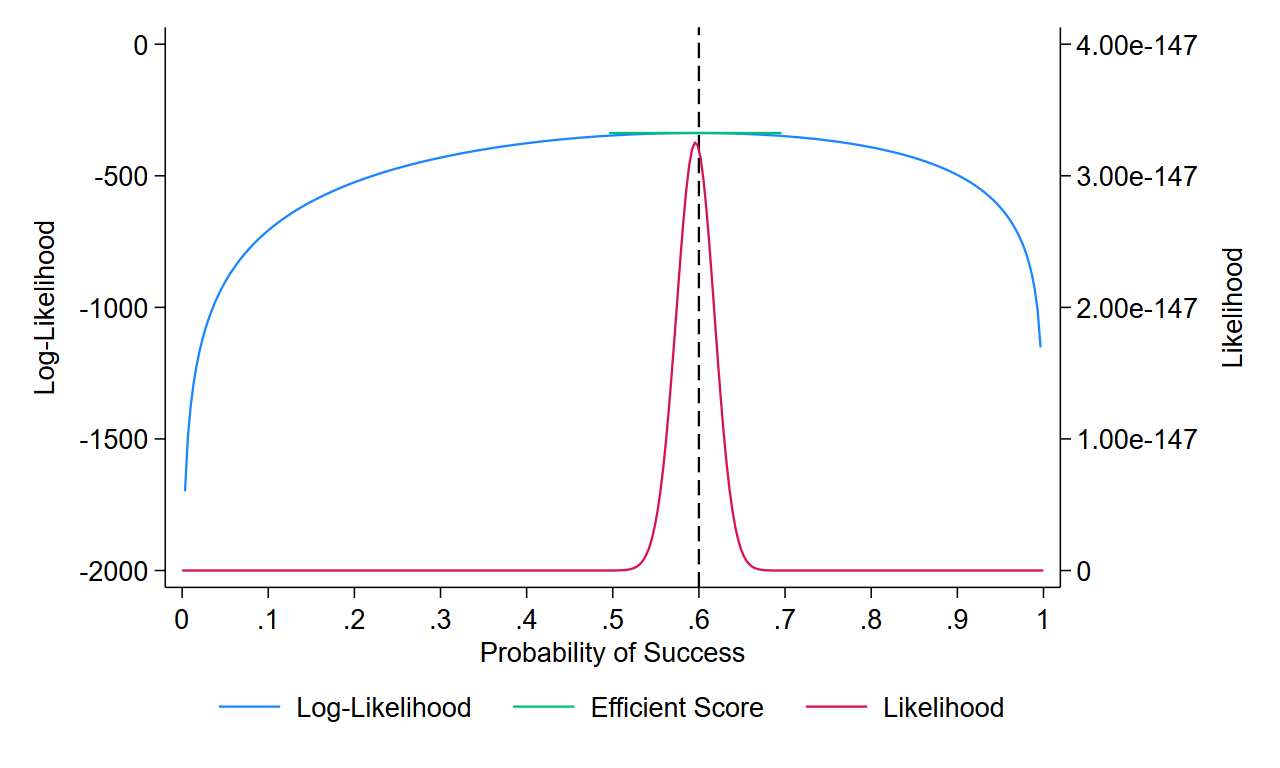
\includegraphics[width=0.6\textwidth]{figures/ll_500}}\label{f1}
\end{center}
\end{figure}
\small
\begin{itemize}
	\item The \textbf{likelihood function} $L_N(\boldsymbol{\theta}|\boldsymbol{y},\boldsymbol{X})$ is the joint probability mass function or density $f(\boldsymbol{y},\boldsymbol{X}|\boldsymbol{\theta})$, viewed as a function of vector $\boldsymbol{\theta}$ given the data $(\boldsymbol{y},\boldsymbol{X})$.

	\item Maximizing $L_N(\boldsymbol{\theta})$ is equivalent to maximizing the \textbf{log-likelihood function} $\mathcal{L}_N(\boldsymbol{\theta)}=\ln L_N(\boldsymbol{\theta})$. Because taking the logarithm is a monotonic transformation. A maximum for $L_N(\boldsymbol{\theta})$ corresponds with a maximum for $\mathcal{L}_N(\boldsymbol{\theta)}$.

\end{itemize}
\end{frame}

\section{The Econometric Model}
\begin{frame}{Specification of a Likelihood Function}
\small
The conditional likelihood $L_N(\boldsymbol{\theta})=f(\boldsymbol{y},\boldsymbol{X}|\boldsymbol{\theta})/f(\boldsymbol{X}|\boldsymbol{\theta})=f(\boldsymbol{y}|\boldsymbol{X},\boldsymbol{\theta})$ does not require the specification of the marginal distribution of $\boldsymbol{X}$.

For observations $(y_i,x_i)$ independent over $i$ and distributed with $f(\boldsymbol{y}|\boldsymbol{X},\boldsymbol{\theta}),$ 
\begin{itemize}
	\item the joint density is $$f(\boldsymbol{y}|\boldsymbol{X},\boldsymbol{\theta})=\Pi_{i=1}^{N}f(y_i|\boldsymbol{x}_i,\boldsymbol{\theta}),$$
	\item the log-likelihood function divided by $N$ is $$\frac{1}{N}\mathcal{L}_N(\boldsymbol{\theta)}=\frac{1}{N}\sum_{i=1}^{N} \ln f(y_i|\boldsymbol{x}_i,\boldsymbol{\theta}).$$
\end{itemize}
\begin{table}
\centering
{
\begin{footnotesize}
\begin{tabular}{@{\extracolsep{4pt}}l*{4}{l}}
\toprule
Model & Range of $y$ & Density $f(y)$ & Common Parametrization\\
\midrule
Bernoulli   & 0 or 1              & $p^y(1-p)^{1-y}$ & $p=\frac{e^{-\bm{x}'\beta}}{1+e^{-\bm{x}'\beta}}$ \\
Poisson     & $0,1,2,\ldots$      & $e^{-\lambda}\lambda^{y}/y!$ & $\lambda=e^{\textbf{x}'\beta}$ \\
Exponential & $(0,\infty)$          & $\lambda e^{-\lambda y}$ & $\lambda=e^{\textbf{x}'\beta}$ or $1/\lambda=e^{\textbf{x}'\beta}$  \\
Normal      & $(-\infty, \infty)$ & $(2\pi\sigma^2)^{-1/2}e^{-(y-\mu)^2/2\sigma^2}$ & $\mu=\bm{x}'\beta,\sigma^2=\sigma^2$ \\
\bottomrule
\end{tabular}
\end{footnotesize}
}
\end{table}

\end{frame}



\begin{frame}{Maximum Likelihood Estimator}

\begin{figure}[H]
\begin{center}
{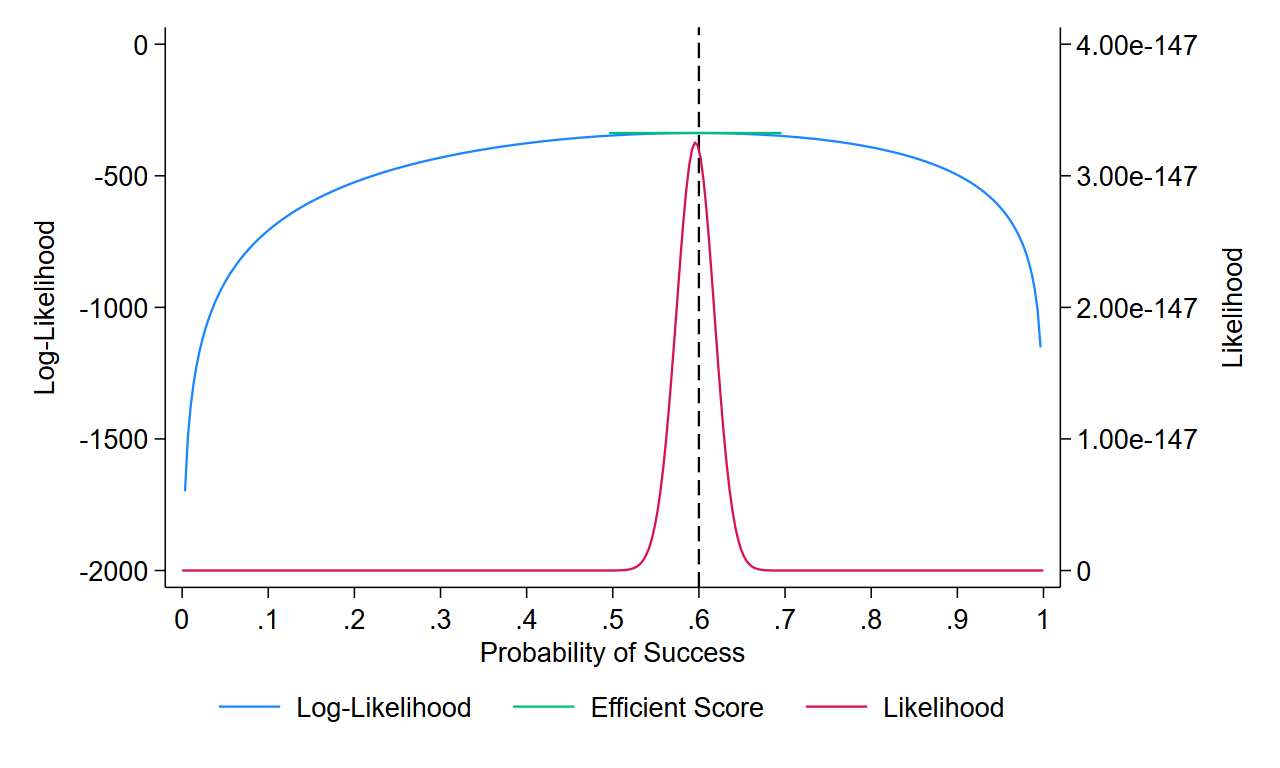
\includegraphics[width=0.6\textwidth]{figures/ll_500}}\label{f1}
\end{center}
\end{figure}
The \textbf{maximum likelihood estimator} (MLE) is the estimator that maximizes the (conditional) log-likelihood function $\mathcal{L}_N(\theta)$.\\ The MLE is the local maximum that solves the first-order conditions
$$\frac{1}{N}\frac{\partial \mathcal{L}_N(\boldsymbol{\theta)}}{\partial \boldsymbol{\theta}}=\frac{1}{N}\sum_{i=1}^{N}\frac{\partial \ln f(y_i|\boldsymbol{x}_i,\boldsymbol{\theta})}{\partial \boldsymbol{\theta}}=\boldsymbol{0}.$$

\end{frame}

\begin{frame}{Maximum Likelihood Estimator}

\begin{figure}[H]
\begin{center}
{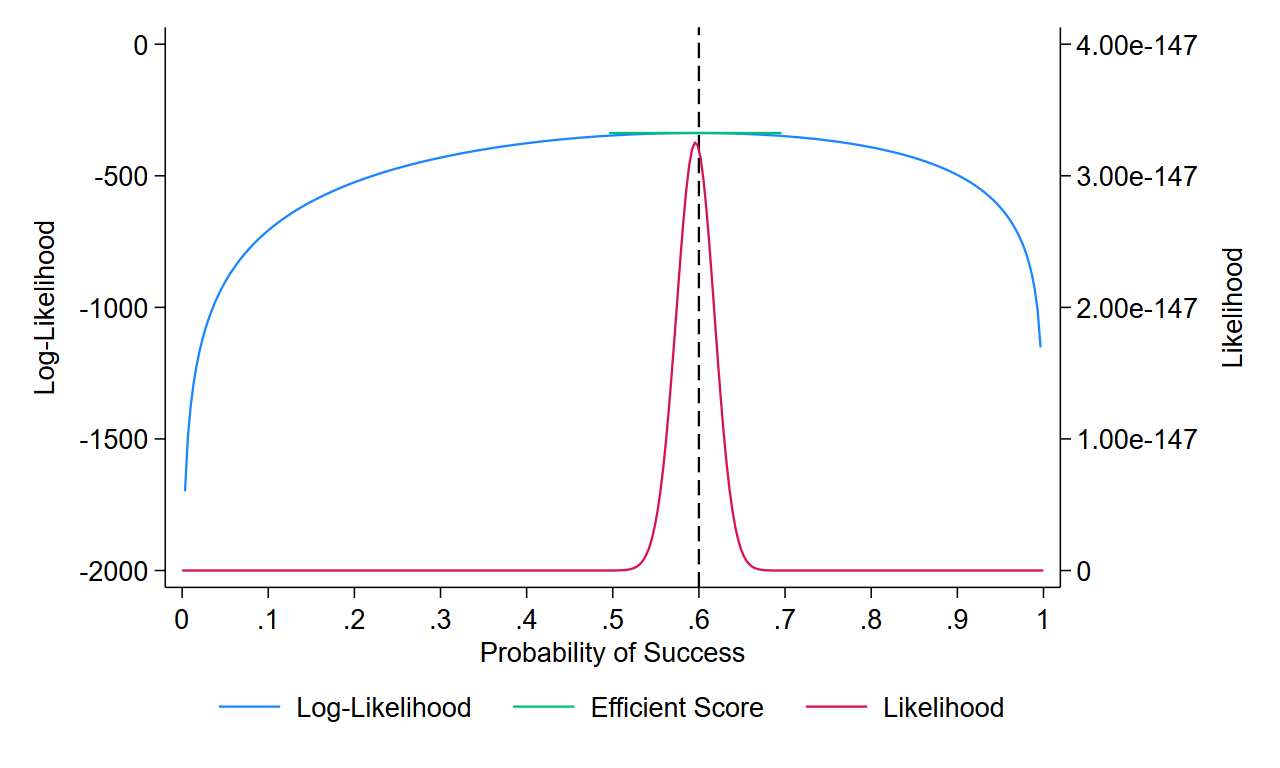
\includegraphics[width=0.6\textwidth]{figures/ll_500}}\label{f1}
\end{center}
\end{figure}
This estimator is an extremum estimator on based on the conditional density of $y$ given $\boldsymbol{x}$.
The gradient vector $\frac{\partial \mathcal{L}_N(\boldsymbol{\theta})}{\partial \boldsymbol{\theta}}$ is called the \textbf{score vector}, as it sums the first derivatives of the log density, and when evaluated at $\boldsymbol{\theta}_0$ it is called the \textbf{efficient score}.\\[4ex]
\quad
\end{frame}



\begin{frame}{How Were the Data Generated?}
\begin{assumption}\small
 \textbf{Simple Random Sampling}. $\{x_{i1},\ldots, x_{iK}, y_i\}^N_{i=1} \quad\text{i.i.d. (independent and identically distributed)}$
\end{assumption}
This assumption means that
\begin{itemize}
	\item observation $i$ has no information content for observation $j\neq i$
	\item all observations $i$ come from the same distribution
\end{itemize}
This assumption is guaranteed by simple random sampling provided there is no systematic non-response or truncation.\\[2ex]


\end{frame}

\begin{frame}{How Were the Data Generated?}

I.i.d. data simplify the maximization as the joint density of the two variables is simply the product of the two marginal densities.\\[2ex] For example with a normal joint pdf with two observations
$$f\left(y_{1}, y_{2}\right)=f_{Y_{1}}\left(y_{1}\right) f_{Y_{2}}\left(y_{2}\right)=\frac{1}{2 \pi \sigma^{2}} e^{-\frac{\left[\left(y_{1}-\mu\right)^{2}+\left(y_{2}-\mu\right)^{2}\right]}{2 \sigma^{2}}}
.$$

With dependent observations we would have to maximize the following likelihood function, where $\rho$ is the correlation:

$$
\frac{1}{2 \pi \sigma^{2} \sqrt{1-\rho^{2}}} e^{-\frac{\left[\left(y_{1}-\mu\right)^{2}+\left(y_{2}-\mu\right)^{2}-\left(y_{1}-\mu\right)\left(y_{2}-\mu\right)\right]}{2 \sigma^{2}\left(1-\rho^{2}\right)}}
.$$
\end{frame}


\begin{frame}{The Score has Expected Value Zero}
Likelihood Equation:
$$E_f\bigg[\boldsymbol{g}(\boldsymbol{\theta})\bigg]=E_f\bigg[\frac{\partial \ln f(y|\boldsymbol{x},\boldsymbol{\theta})}{\partial \boldsymbol{\theta}}\bigg]=\int\frac{\partial \ln f(y|\boldsymbol{x},\boldsymbol{\theta})}{\partial \boldsymbol{\theta}} f(y|\boldsymbol{x},\boldsymbol{\theta})dy=\boldsymbol{0}.$$
\footnotesize
\begin{example}
 
$$\int f(y|\boldsymbol{\theta})dy=1. \quad \frac{\partial}{\partial \boldsymbol{\theta}}\int f(y|\boldsymbol{\theta})dy=0.$$
$$\int\frac{\partial f(y|\boldsymbol{\theta})}{\partial \boldsymbol{\theta}} dy=0.$$

$$\partial \ln f(y|\boldsymbol{\theta})/\partial \boldsymbol{\theta}=[\partial f(y|\boldsymbol{\theta})/\partial \boldsymbol{\theta}]/[f(y|\boldsymbol{\theta})]$$

$$\frac{\partial f(y|\boldsymbol{\theta})}{\partial \boldsymbol{\theta}}=\frac{\partial \ln f(y|\boldsymbol{\theta})}{\partial \boldsymbol{\theta}}f(y|\boldsymbol{\theta}).$$

$$\int\frac{\partial \ln f(y|\boldsymbol{\theta})}{\partial \boldsymbol{\theta}} f(y|\boldsymbol{\theta})dy=0.$$
\end{example}
\end{frame}

\begin{frame}{Fisher Information}
The information matrix is the expectation of the outer product of the score vector,
$$\mathcal{I}=E_f\bigg[\frac{\partial \ln f(y|\boldsymbol{x},\boldsymbol{\theta})}{\partial \boldsymbol{\theta}}\frac{\partial \ln f(y|\boldsymbol{x},\boldsymbol{\theta})}{\partial \boldsymbol{\theta}'}\bigg].$$

The Fisher information $\mathcal{I}$ is equals the variance of the score, since $\frac{\partial \mathcal{L}_N(\boldsymbol{\theta})}{\partial \boldsymbol{\theta}}$ has mean zero.
\begin{itemize}
	\item Large values of $\mathcal{I}$ mean that small changes in $\boldsymbol{\theta}$ lead to large changes in the log-likelihood \\$\rightarrow \mathcal{L}_N(\boldsymbol{\theta})$ contains considerable
information about $\boldsymbol{\theta},$
	\item Small values of $\mathcal{I}$ mean that the maximum is shallow and there are many nearby values of $\boldsymbol{\theta}$ with a similar log-likelihood.
\end{itemize}
\end{frame}


\begin{frame}{Information Matrix Equality}
\small
The Fisher information $\mathcal{I}$ is equals the expectation of the Hessian $\boldsymbol{H}$:
$$-E_f\bigg[\boldsymbol{H}(\boldsymbol{\theta})\bigg]=-E_f\bigg[\frac{\partial^2 \ln f(y|\boldsymbol{x},\boldsymbol{\theta})}{\partial \boldsymbol{\theta}\partial\boldsymbol{\theta}'}\bigg]=E_f\bigg[\frac{\partial \ln f(y|\boldsymbol{x},\boldsymbol{\theta})}{\partial \boldsymbol{\theta}}\frac{\partial \ln f(y|\boldsymbol{x},\boldsymbol{\theta})}{\partial \boldsymbol{\theta}'}\bigg].$$
\footnotesize

\begin{example}
\vspace{-5mm}
$$\text{For vector moment function, e.g., } \boldsymbol{m}(y,\boldsymbol{\theta})=\frac{\partial \ln f(y|\boldsymbol{\theta})}{\partial \boldsymbol{\theta}} \text{ with } E[\boldsymbol{m}(y,\boldsymbol{\theta})]=0,$$
$$\int \boldsymbol{m}(y,\boldsymbol{\theta})f(y|\boldsymbol{\theta})dy=0.$$

$$\int\bigg(\frac{\partial \boldsymbol{m}(y,\boldsymbol{\theta})}{\partial \boldsymbol{\theta}'} f(y|\boldsymbol{\theta})+\boldsymbol{m}(y,\boldsymbol{\theta})\frac{\partial f(y|\boldsymbol{\theta})}{\partial \boldsymbol{\theta}'}\bigg)dy=0.$$

$$\int\bigg(\frac{\partial \boldsymbol{m}(y,\boldsymbol{\theta})}{\partial \boldsymbol{\theta}'} f(y|\boldsymbol{\theta})+\boldsymbol{m}(y,\boldsymbol{\theta})\frac{\partial \ln f(y|\boldsymbol{\theta})}{\partial \boldsymbol{\theta}'}f(y|\boldsymbol{\theta})\bigg)dy=0.$$

$$E\bigg[\frac{\partial \boldsymbol{m}(y,\boldsymbol{\theta})}{\partial \boldsymbol{\theta}'}\bigg]=-E\bigg[\boldsymbol{m}(y,\boldsymbol{\theta})\frac{\partial \ln f(y|\boldsymbol{\theta})}{\partial \boldsymbol{\theta}'}\bigg] =0.$$

\end{example}
\end{frame}



\begin{frame}
\frametitle{The Information Matrix in Practice}
\footnotesize

The variance of the sum of random score vector is:

\textbf{Information matrix equality:}
$$
\operatorname{Var}\left[\sum_{i=1}^{n} \boldsymbol{g}_{i}\left(\boldsymbol{\theta}\right)\right]=\operatorname{Var}\left[\boldsymbol{g}\left(\boldsymbol{\theta}\right)\right]=-E_f\left[\boldsymbol{H}\left(\boldsymbol{\theta}\right)\right]=-E\left[\frac{\partial^{2} \ln L}{\partial \boldsymbol{\theta} \partial \boldsymbol{\theta}^{\prime}}\right].
$$

After taking the expected value, $\widehat{\boldsymbol{\theta}}$ is substituted for $\boldsymbol{\theta}$. Problem: Taking the expected value of the second derivative matrix is frequently infeasible.\\[2ex]

There exist two alternatives which are asymptotically equivalent:
\begin{itemize}
	\item Ignore the expected value operator:

$$
\widehat{\boldsymbol{I}}(\widehat{\boldsymbol{\theta}})=-\frac{\partial^{2} \ln L}{\partial \widehat{\boldsymbol{\theta}} \partial \widehat{\boldsymbol{\theta}}^{\prime}}.
$$
	\item Berndt-Hall-Hall-Hausman (BHHH) algorithm\\ Never take a second derivative and sum over the outer product of the scores: (first derivatives per observation):
$$
\check{\boldsymbol{I}}(\widehat{\boldsymbol{\theta}})=\sum_{i=1}^{n} \widehat{\boldsymbol{g}}_{i} \widehat{\boldsymbol{g}}_{i}^{\prime}=\sum_{i=1}^{n}\left(\frac{\partial \ln f\left(y_{i}, \widehat{\boldsymbol{\theta}}\right)}{\partial \widehat{\boldsymbol{\theta}}}\right)\left(\frac{\partial \ln f\left(y_{i}, \widehat{\boldsymbol{\theta}}\right)}{\partial \widehat{\boldsymbol{\theta}}}\right)^{\prime}.
$$
\end{itemize}

\end{frame}

\section{Properties of the Maximum Likelihood Estimator}

\begin{frame}{Properties of the MLE}


\begin{itemize}
	\item \emph{Small sample properties of $\hat{\boldsymbol{\theta}}$}
\begin{itemize}
	\item may be biased
	\item may have unknown distribution
	\item variance may be biased, even towards zero\\[4ex]
\end{itemize}
	\item \emph{Large sample properties of $\hat{\boldsymbol{\theta}}$}
\begin{itemize}
	\item consistent
	\item approx. normal
	\item asymptotically efficient
	\item invariant
\end{itemize}
\end{itemize}


\end{frame}

\begin{frame}{Consistency}
%\beamerdefaultoverlayspecification{<+->}
\begin{columns}
\begin{column}{0.45\textwidth}
\small
\textbf{Law of Large Numbers}\\\pause
As $N$ increases, the distribution of $\hat{\boldsymbol{\theta}}$ becomes more tightly centered around $\boldsymbol{\theta}$.\pause
\end{column}
\begin{column}{0.55\textwidth}  %%<--- here
%-------------------------------------------
\begin{figure}[htbp]
	\begin{subfigure}[c]{0.49\textwidth}
		\centering
		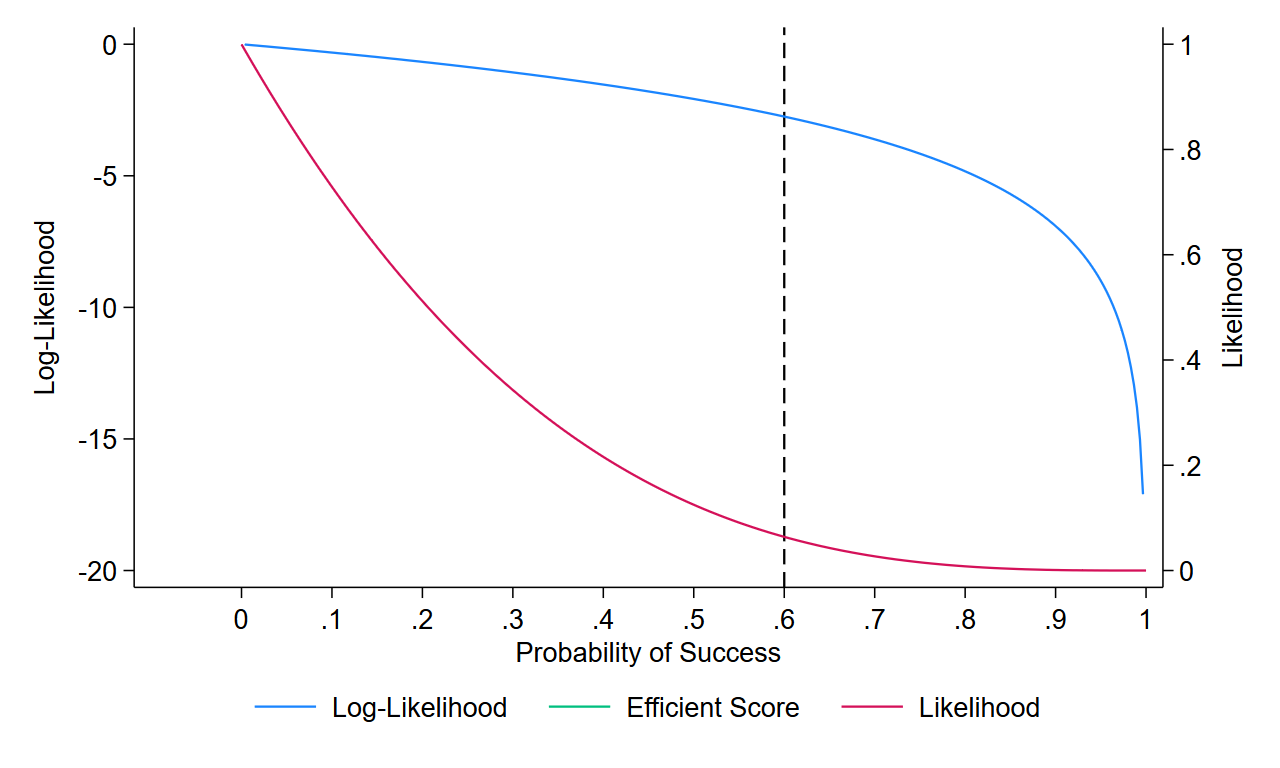
\includegraphics[width=1\textwidth]{figures/ll_3}
		\caption{N=3}
    \label{fig:distribution beta1 N3}
	\end{subfigure}%
	\pause
	\begin{subfigure}[c]{0.49\textwidth}
		\centering
		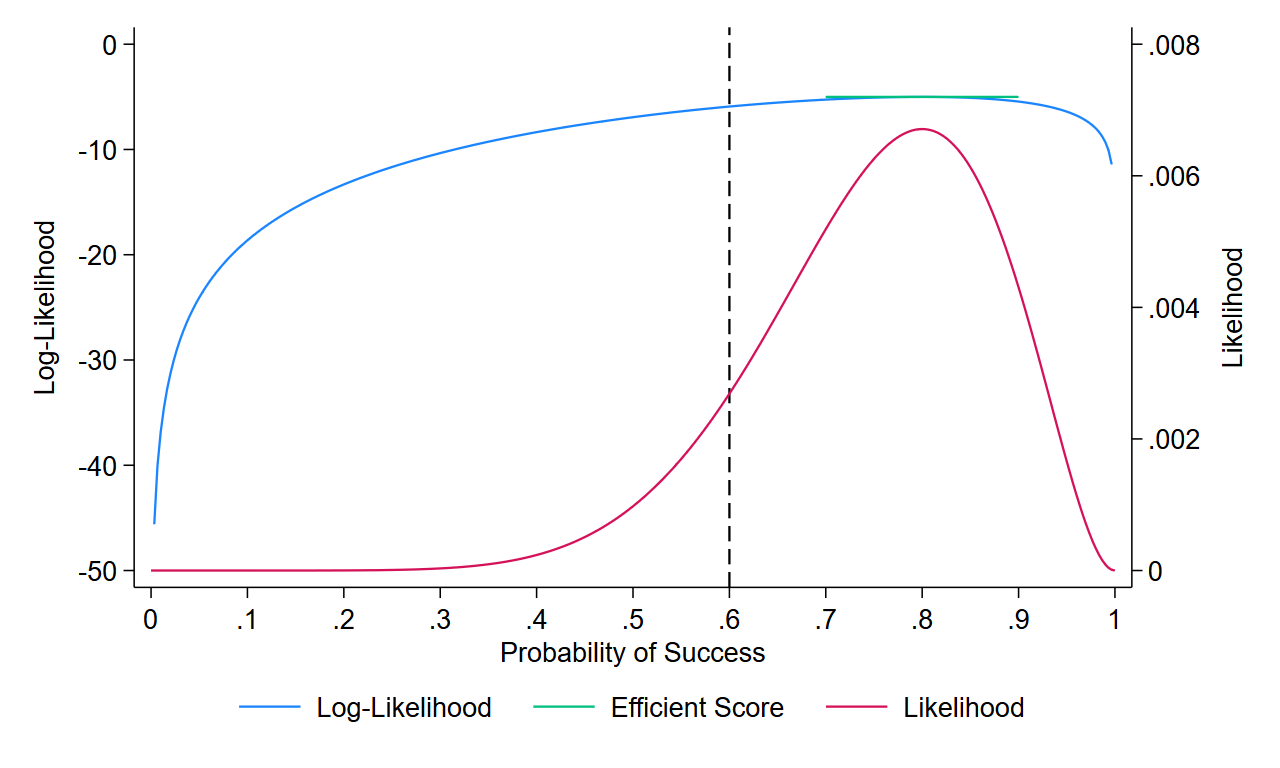
\includegraphics[width=1\textwidth]{figures/ll_10}
		\caption{N=10}
		\label{fig:distribution beta1 N10}								
	\end{subfigure}\\
	\pause
	\begin{subfigure}[c]{0.49\textwidth}
		\centering
		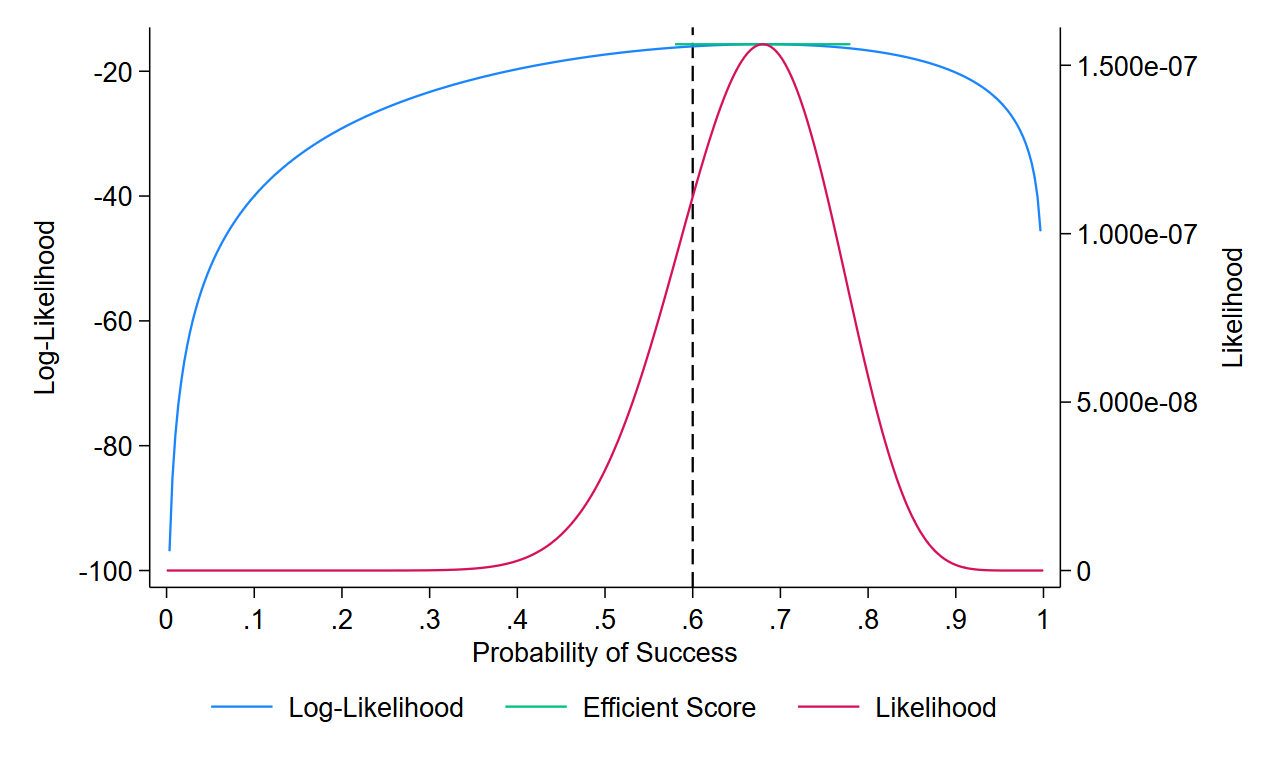
\includegraphics[width=1\textwidth]{figures/ll_25}
		\caption{N=25}
		\label{fig:distribution beta1 N25}								
  \end{subfigure}
	\pause
	\begin{subfigure}[c]{0.49\textwidth}
		\centering
		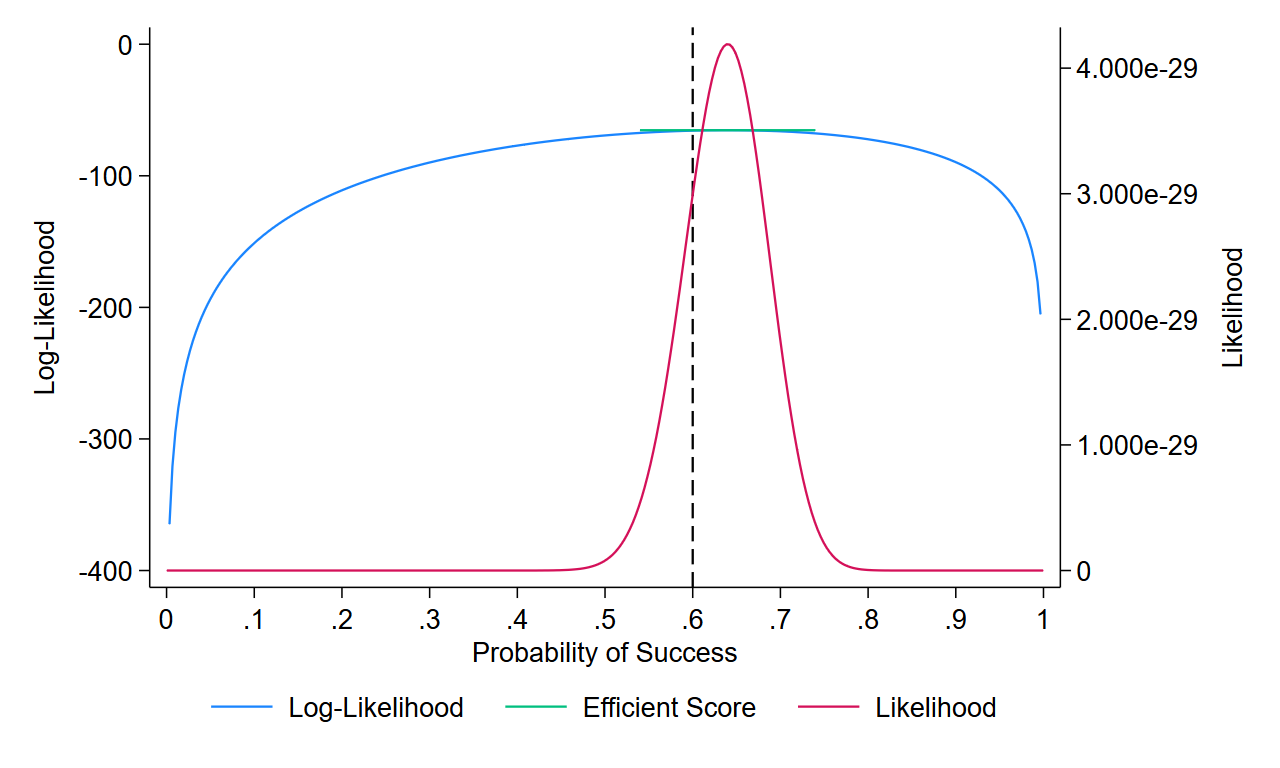
\includegraphics[width=1\textwidth]{figures/ll_100}
		\caption{N=100}
		\label{fig:distribution beta1 N100}								
  \end{subfigure}
%\caption{Distribution of beta1}
\end{figure} 
%-------------------------------------------
\end{column}
\end{columns}

\end{frame}

\begin{frame}{Consistency}

Likelihood Inequality\pause
$$E[(1/N)\ln L(\hat{\boldsymbol{\theta}})]\geq E[(1/N)\ln L(\boldsymbol{\theta})].$$\pause

The expected value of the log-likelihood is maximized at the true value of the parameters.\pause

\begin{figure}[t]
	\centering
{		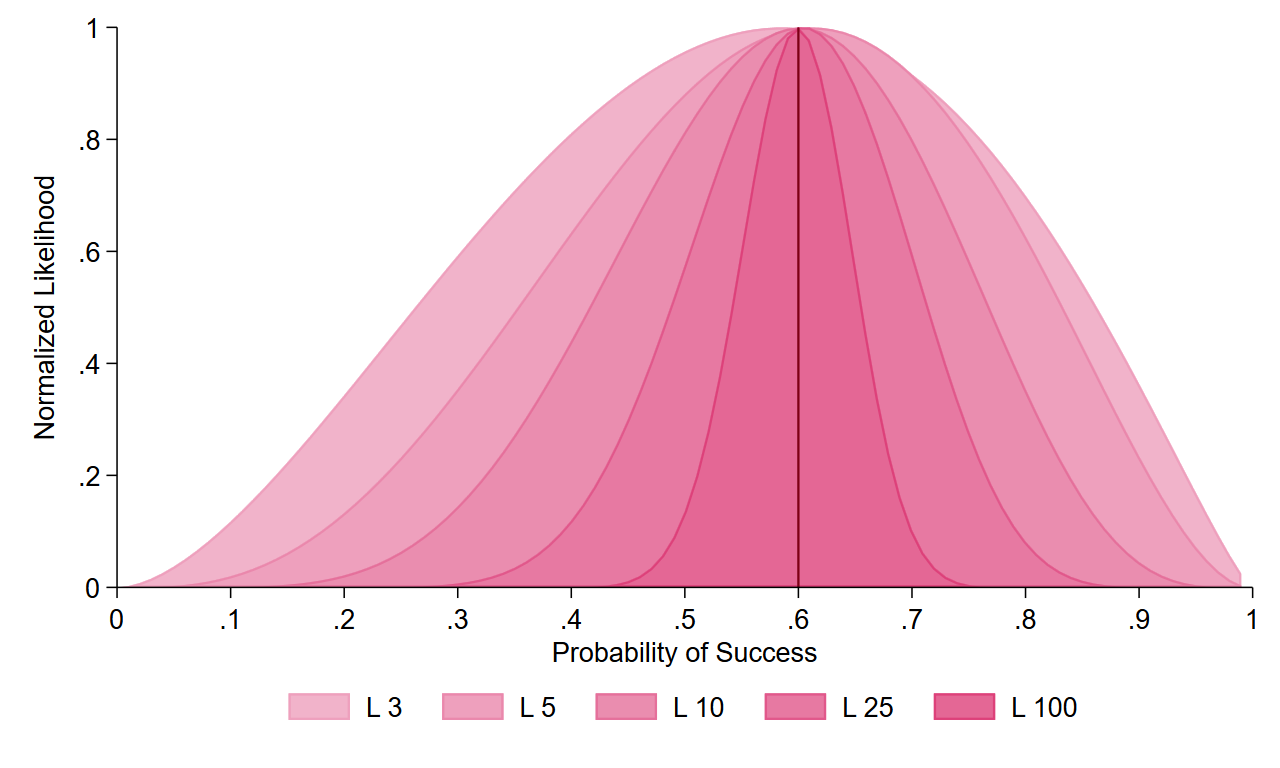
\includegraphics[width=.4\textwidth]{figures/l.png}}\pause
{		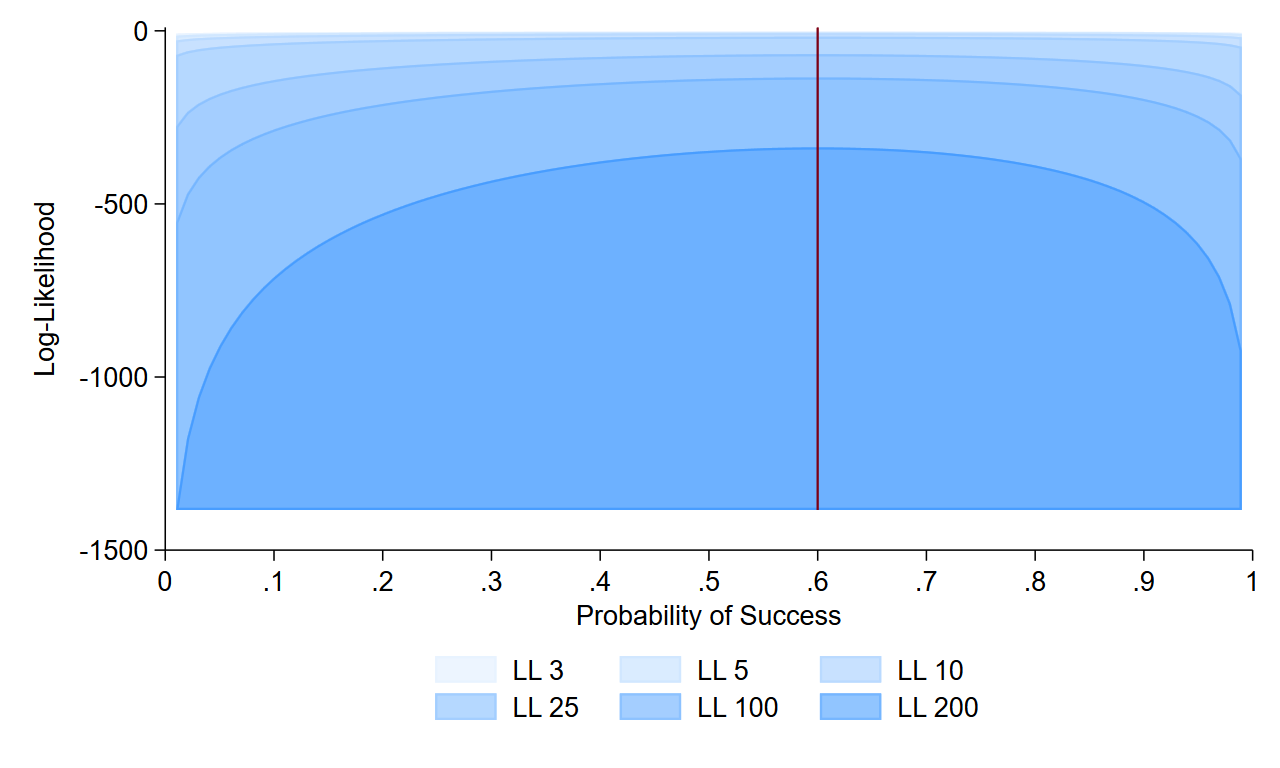
\includegraphics[width=.4\textwidth]{figures/ll.png}}\pause
	\caption{$\hat{\theta}$, Likelihood and Log-Likelihood as $n\rightarrow\infty$. True $\theta=0.6$.
	}
\end{figure}	\pause
	
$$\lim_{n\rightarrow\infty}P(|\hat{\boldsymbol{\theta}}-\boldsymbol{\theta}|>\epsilon)=\boldsymbol{0}.\pause  \quad\quad
\lim_{n\rightarrow\infty}E[\hat{\boldsymbol{\theta}}]=\boldsymbol{\theta}.$$
	
\end{frame}

\begin{frame}{Approximate Normality}
\textbf{Central Limit Theorem}\\
As $N$ becomes large, 
$$\hat{\boldsymbol{\theta}}\overset{\text{a}}{\sim} N\bigg[\boldsymbol{\theta}, -\left(E\bigg[\frac{\partial^2 \mathcal{L}_N(\boldsymbol{\theta})}{\partial\boldsymbol{\theta}\partial\boldsymbol{\theta}'}\bigg]\right)^{-1}\bigg].$$
	
	
\begin{figure}[t]
	\centering
{		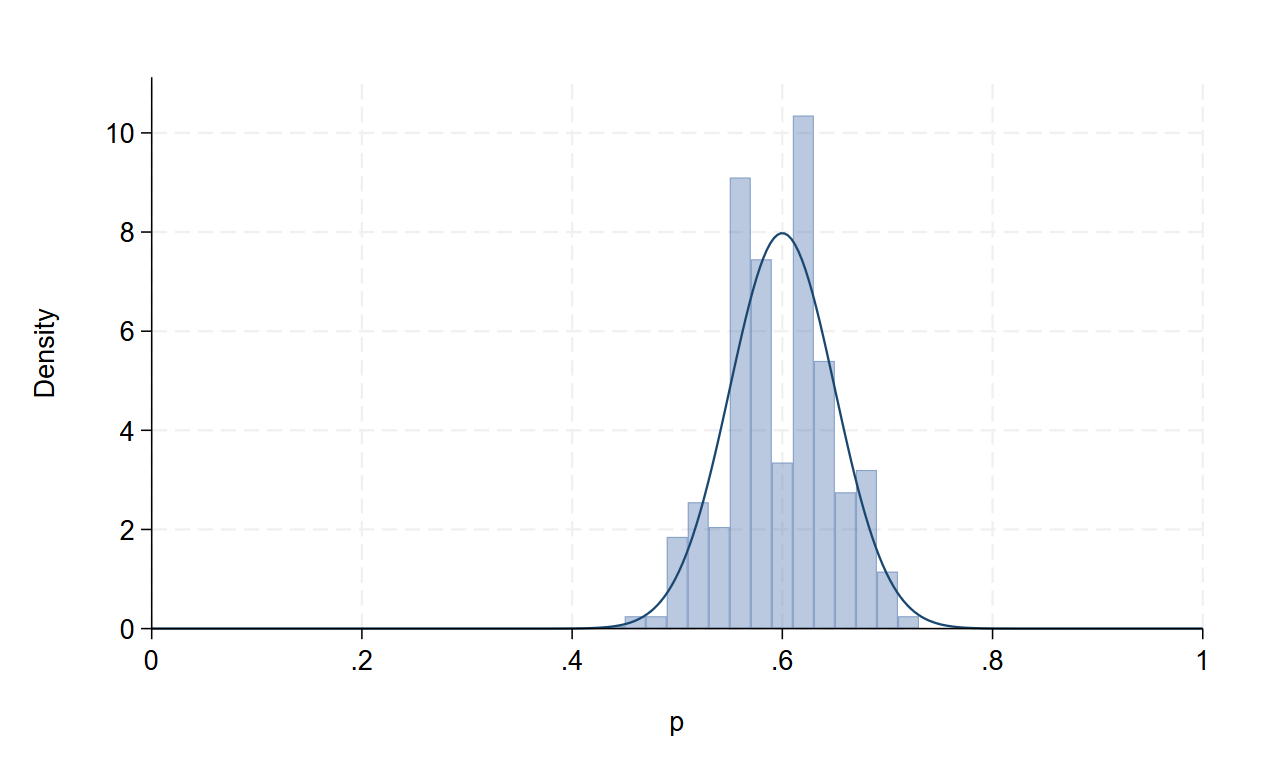
\includegraphics[width=.55\textwidth]{figures/distribution_p_100.png}}
	\caption{Sampling distribution of $\hat{\boldsymbol{\theta}}$ drawn from Bernoulli distribution and normal distribution at $N=100$. True $\boldsymbol{\theta}=0.6$.
	}
\end{figure}	
	
\end{frame}




\begin{frame}{Efficiency}
\footnotesize The precision of the estimate $\hat{\boldsymbol{\theta}}$ is limited by the Fisher information $\mathcal{I}$ of the likelihood.
$$
\operatorname{Var}\left(\hat{\boldsymbol{\theta}}\right) \geq \frac{1}{\mathcal{I}\left(\boldsymbol{\theta}\right)}.
$$

For large samples, this is the so-called Cram\'{e}r-Rao lower bound for the variance matrix of consistent asymptotically normal estimators with convergence to normality of $\sqrt{N}(\hat{\boldsymbol{\theta}}-\boldsymbol{\theta}_0)$ uniform in compact intervals of $\boldsymbol{\theta}_0$.

Under the strong assumption of correct specification of the conditional density, the MLE has the \textbf{smallest asymptotic variance} among root-$N$ consistent estimators.
\begin{example}
\footnotesize
 Since the MLE is unbiased, 
$$
\operatorname{E}\left[ \left. \hat{\boldsymbol{\theta}} - \boldsymbol{\theta} \,\, \right| \,\, \boldsymbol{\theta} \right]
= \int \left(\hat{\boldsymbol{\theta}} - \boldsymbol{\theta}\right) \, f(y ;\boldsymbol{\theta}) \, dy = 0 \text{ regardless of the value of } \boldsymbol{\theta}.
$$

This expression is zero independent of $\boldsymbol{\theta}$, so its partial derivative with respect to $\boldsymbol{\theta}$ must also be zero. By the product rule, this partial derivative is also equal to

$$
0 = \frac{\partial}{\partial\boldsymbol{\theta}} \int \left(\hat{\boldsymbol{\theta}} - \boldsymbol{\theta} \right) \, f(y ;\boldsymbol{\theta}) \,dy
= \int \left(\hat{\boldsymbol{\theta}}-\boldsymbol{\theta}\right) \frac{\partial f}{\partial\boldsymbol{\theta}} \, dy - \int f \,dy.
$$


\end{example}


\end{frame}


\begin{frame}{Efficiency}

\begin{example}
\scriptsize
 
For each $\boldsymbol{\theta}$, the likelihood function is a probability density function, and therefore $\int f\,dy = 1$. By using the chain rule on the partial derivative of $\ln f$ and then dividing and multiplying by $f(y;\boldsymbol{\theta})$, one can verify that

$$\frac{\partial f}{\partial\boldsymbol{\theta}} = f \, \frac{\partial \ln f}{\partial\boldsymbol{\theta}}.$$
Using these two facts, we get

$$
\int \left(\hat{\boldsymbol{\theta}}-\boldsymbol{\theta}\right) f \, \frac{\partial \ln f}{\partial\boldsymbol{\theta}} \, dy = 1.
$$

Factoring the integrand gives$
\int \left(\left(\hat{\boldsymbol{\theta}}-\boldsymbol{\theta}\right) \sqrt{f} \right) \left( \sqrt{f} \, \frac{\partial \ln f}{\partial\boldsymbol{\theta}} \right) \, dy = 1.
$

Squaring the expression in the integral, the Cauchy-Schwarz inequality yields

$$
1 =
\biggl( \int \left[\left(\hat{\boldsymbol{\theta}}-\boldsymbol{\theta}\right) \sqrt{f} \right] \cdot \left[ \sqrt{f} \, \frac{\partial \ln f}{\partial\boldsymbol{\theta}} \right] \, dy \biggr)^2
\le
\left[ \int \left(\hat{\boldsymbol{\theta}} - \boldsymbol{\theta}\right)^2 f \, dy \right] \cdot \left[ \int \left( \frac{\partial \ln f}{\partial\boldsymbol{\theta}} \right)^2 f \, dy \right].
$$

The first factor is the expected mean-squared error (the variance) of the estimator $\hat{\boldsymbol{\theta}}$, the second factor is the Fisher Information.
\end{example}


\end{frame}

\begin{frame}{Invariance}
\small The MLE of $\boldsymbol{\gamma}=\boldsymbol{c}\left(\boldsymbol{\theta}\right)$ is $\widehat{\boldsymbol{\theta}}=\boldsymbol{c}(\widehat{\boldsymbol{\theta}})$ if $\boldsymbol{c}\left(\boldsymbol{\theta}\right)$ is a continuous and continuous differentiable function.


\begin{itemize}
	\item This simplifies the log-likelihood,
	\item This allows a function of $\widehat{\boldsymbol{\theta}}$ to serve as MLE if it is desired to analyze the function of an MLE.
\end{itemize}
\begin{example}
\footnotesize
Suppose that the normal log-likelihood is parameterized in terms of the precision parameter, $\theta^2 = 1/\sigma^2$. The log-likelihood becomes
$$\ln L(\mu, \sigma^2)=-(N/2)\ln(2\pi)+(N/2)\ln\theta^2-\frac{\theta^2}{2}\sum_{i=1}^N(y_i-\mu)^2.$$
The MLE for $\mu$ is $\bar{x}$. But the likelihood equation for $\theta^2$ is now
$$\frac{\partial \ln L(\mu, \theta^2)}{\partial \theta^2}=1/2\bigg[N/\theta^2-\sum_{i=1}^N(y_i-\mu)^2\bigg]=0,$$
which has solution $\hat{\theta}^2 =N/\sum_{i=1}^N(y_i - \mu)^2 =1/\hat{\sigma}^2$.

\end{example}

\end{frame}



\begin{frame}{Invariance}

The MLE is also equivariant with respect to certain \textbf{transformations of the data}.\\[2ex]

If $y=c(x)$ where $c$ is one to one and does not depend on the parameters to be estimated, then the density functions satisfy

$$f_Y(y) = \frac{f_X(x)}{|c'(x)|},$$

and hence the likelihood functions for $x$ and $y$ differ only by a factor that does not depend on the model parameters.

\begin{example}
The MLE parameters of the log-normal distribution are the same as those of the normal distribution fitted to the logarithm of the data.
\end{example}

\end{frame}




\begin{frame}[t,allowframebreaks
]\nocite{*}
\frametitle{References}
\small
\bibliography{bib}
\end{frame}


\end{document}
